\begin{figure*}[t]
  \centering
  \begin{minipage}{0.33\textwidth}
    \centering
    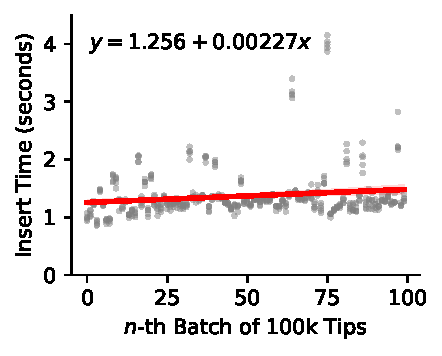
\includegraphics[height=4.3cm]{img/series-purifying.pdf}
    \vspace{-0.5em}
    \subcaption{Purifying Regime}
    \label{fig:scaling:purifying}
  \end{minipage}%
  \begin{minipage}{0.33\textwidth}
    \centering
    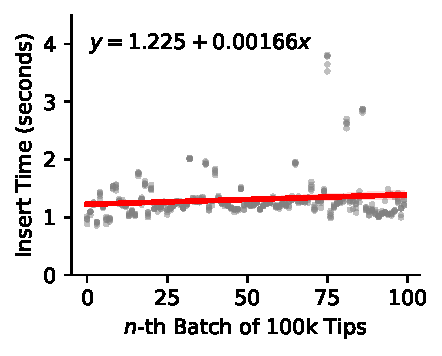
\includegraphics[height=4.3cm,trim={0.7cm 0 0 0},clip]{img/series-adaptive.pdf}
    \vspace{-0.5em}
    \subcaption{Adaptive Regime}
    \label{fig:scaling:adaptive}
  \end{minipage}%
  \begin{minipage}{0.33\textwidth}
    \caption{%
    \textbf{Empirical performance scaling of shortcut table algorithm in microbenchmark trials.}
    \footnotesize
    Panels \ref{fig:scaling:purifying} and \ref{fig:scaling:adaptive} differ in simulation data source of sampled genomes, with the former exhibiting higher phylogenetic richness. Data collected as batches are added in a 10 million tip reconstruction, sampled 5 times per panel.
    Adapted from \citet{singhvi2025scalable}.
}
    \label{fig:scaling}
  \end{minipage}
  \vspace{-1.5em}
\end{figure*}
